\subsubsection{Key Storage - Online and Caching} \label{section:counter-replace-encryption-key-online}
The first approach to handle the encryption key is to store it on a server and provide it to the application.
This works similar to the license verification.
\newline
On decrypt method call, the application tries to retrieve a cached cryptographic key.
In case a cached key is available, the application starts to decrypt the content.
Otherwise the key is requested from the server.
The server does a verification of the user similar to the license verification libraries.
In case the check is successful, the decryption key is send to the device instead of a simple yes or no.
The advantage over having the original implementation is that the key can neither be accessed without the verification on the server and nor guessed by an attacker to circumvent this countermeasure.
\newline
The key can either be retrieved from the server for each decryption action or it can be cached on the device, similar to the license verification policy.
Caching should be favored since getting the key for each action not only requires to be online but slows down the application and generates additional traffic.
\newline
In order to improve security, keys can be changed when updating the version of the application or be user specific.
\begin{figure}[h]
    \centering
    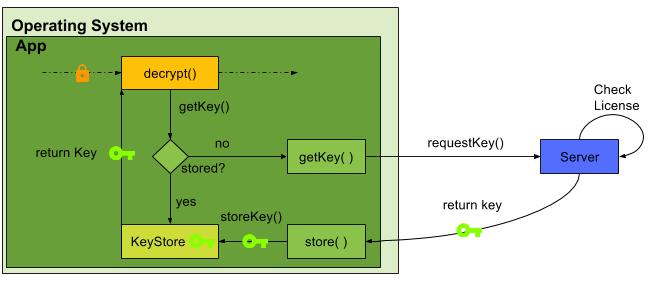
\includegraphics[width=0.8\textwidth]{data/encryptionKeyServer.png}
    \caption{Retrieving the key after successful identification from the server and store it local on device}
    \label{fig:encryptionKeyServer}
\end{figure}
